\documentclass[10pt, a4paper, landscape, xcolor=dvipsnames]{extarticle}
\pagestyle{empty} % Keine Seitennummern

% Verwendete Pakete

	\usepackage[utf8]{inputenc}
	\usepackage[top=0.7cm, bottom=0.9cm, left=0.65 cm, right=0.65 cm, ]{geometry}
	\usepackage{amsmath}
	\usepackage{amsfonts}
	\usepackage{lmodern}
	\usepackage{graphicx}
	\setlength{\parindent}{0pt}
	\usepackage[normalem]{ulem}
	\usepackage[dvipsnames]{xcolor}
	\usepackage{enumitem}
	\usepackage{mathabx}
	\usepackage{enumitem}
	\usepackage{colortbl}
	\usepackage[ngerman]{babel}
	\usepackage{mathtools}
	\usepackage{wallpaper}
	\usepackage{changepage}
	\usepackage{tikz}
	\usepackage{tabularx}
	\usepackage{tcolorbox}
	\usepackage{lipsum}
	\usepackage{multicol}
	\usepackage{letltxmacro}
	\usepackage{tabularx}
	\usepackage{multicol}
	\usepackage{multicol}
	\usepackage{calc}
	\usepackage{ifthen}
	\usepackage{hyperref}
	\usepackage{graphicx}
	\graphicspath{ {./img/} }
	\usepackage{wrapfig}


% Spalteneinstellungen

	\setlength\columnsep{3mm}
	\setlength{\columnseprule}{0pt}
	
% Neue Befehle

	% Bullet-Symbol für Aufzählungen
	\renewcommand\textbullet{\ensuremath{\bullet}}
	
	% Eingekreiste Nummern für Aufzählungen
	\newcommand*\circled[1]{\tikz[baseline=(char.base)]{
            \node[shape=circle,draw,inner sep=1.2pt] (char) {#1};}}
            
    % Horizontale Punkte
    \LetLtxMacro\orgddots\ddots
    \makeatletter
	\DeclareRobustCommand\vdots{%
	  \mathpalette\@vdots{}%
	}
	\newcommand*{\@vdots}[2]{%
	  % #1: math style
	  % #2: unused
	  \sbox0{$#1\cdotp\cdotp\cdotp\m@th$}%
	  \sbox2{$#1.\m@th$}%
	  \vbox{%
	    \dimen@=\wd0 %
	    \advance\dimen@ -3\ht2 %
	    \kern.5\dimen@
	    % remove side bearings
	    \dimen@=\wd2 %
	    \advance\dimen@ -\ht2 %
	    \dimen2=\wd0 %
	    \advance\dimen2 -\dimen@
	    \vbox to \dimen2{%
	      \offinterlineskip
	      \copy2 \vfill\copy2 \vfill\copy2 %
	    }%
	   }%
	}
	\DeclareRobustCommand\ddots{%
		\mathinner{%
		   \mathpalette\@ddots{}%
		   \mkern\thinmuskip
		}%
	}
	
	% Vertikale Punkte
	\DeclareRobustCommand\ddots{%
		  \mathinner{%
		    \mathpalette\@ddots{}%
		    \mkern\thinmuskip
		  }%
		}
		\newcommand*{\@ddots}[2]{%
		  % #1: math style
		  % #2: unused
		  \sbox0{$#1\cdotp\cdotp\cdotp\m@th$}%
		  \sbox2{$#1.\m@th$}%
		  \vbox{%
		    \dimen@=\wd0 %
		    \advance\dimen@ -3\ht2 %
		    \kern.5\dimen@
		    % remove side bearings
		    \dimen@=\wd2 %
		    \advance\dimen@ -\ht2 %
		    \dimen2=\wd0 %
		    \advance\dimen2 -\dimen@
		    \vbox to \dimen2{%
		      \offinterlineskip
		      \hbox{$#1\mathpunct{.}\m@th$}%
		      \vfill
		      \hbox{$#1\mathpunct{\kern\wd2}\mathpunct{.}\m@th$}%
		      \vfill
		      \hbox{$#1\mathpunct{\kern\wd2}\mathpunct{\kern\wd2}\mathpunct{.}\m@th$}%
		    }%
		  }%
		}
	\makeatother
	
	% Schriftart
	\renewcommand{\familydefault}{\sfdefault}
	
	% Dokument-Info Block	
	\newcommand{\DocumentInfo}[3]{
	\begin{tcolorbox}[
			arc=0mm, 
			colback = white!38!black,
			boxrule=0pt,
			toptitle=1mm,
			bottomtitle=1mm,
			right=2mm,
			left=2mm,
			leftright skip = -0.5mm,
			title= \huge \center \textbf{#1} \par \large \vskip1mm #2 \par \vskip1mm \small 	Version: \today,
			fontupper=\color{white},
			after skip = 0 mm,
			top=0.1mm,
			bottom=1mm]
		
		\small #3
	\vskip1mm	
	\end{tcolorbox}
	}
	
	% Überschrift
	\renewcommand{\section}[1]{
	\begin{tcolorbox}[
			arc=0mm,
			colback=white!38!black,
			colframe=white,
			bottomrule = 0 mm,
			toprule = 0 mm,
			leftrule = 0 mm,
			rightrule = 0 mm,
			valign=center,
			left=0.5mm,
			top= 0.7 mm,
			bottom= 0.7 mm,
			fontupper=\color{white},
			before skip = 0mm,
			leftright skip = -0.5mm,
			after skip = 0 mm]

		\textbf{#1}
	\end{tcolorbox}
	}
	
	% Abschnitt	
	\renewcommand{\subsection}[2]{
	\begin{tcolorbox}[
			arc=0mm,
			colback=white!75!black,
			colframe=white,
			bottomrule = 0 mm,
			toprule = 0 mm,
			leftrule = 0 mm,
			rightrule = 0 mm,
			valign=center,
			left=0.5mm,
			top=0.2mm,
			bottom=0.2mm,
			before skip = 0mm,
			leftright skip = -0.5mm,
			after skip = 1.4 mm]
			
		\small \textbf{#1}
	\end{tcolorbox}
	
	\begin{adjustwidth}{0.5mm}{1mm}
		\small
		#2
		\vspace{0.5mm}
	\end{adjustwidth}
	}
	
	% Weisser Balken zwischen Abschnitten
	\newcommand{\WhiteSpace}[0]{
	\begin{tcolorbox}[
			arc=0mm,
			colback=white,
			colframe=white,
			bottomrule = 0 mm,
			toprule = 0 mm,
			leftrule = 0 mm,
			rightrule = 0 mm,
			valign=center,
			left=0.5mm,
			top= -0.2 mm,
			bottom= -0.2 mm,
			fontupper=\color{white},
			before skip = 0mm,
			leftright skip = -0.5mm,
			after skip = 0 mm]
	
	\end{tcolorbox}
	}
	
% Hintergrundbild (graue Spalten)

%	\CenterWallPaper{1}{0_Setup/background.pdf}

% TabularX Zeug (Paket für Tabellen)

	\newcolumntype{C}[1]{>{\centering\arraybackslash}p{#1}}

% TikZ Zeug (Paket für Vektorgraphiken)

	\usetikzlibrary{decorations.pathreplacing,calc}

	\newcommand{\tikzmark}[2][-3pt]{\tikz[remember picture, overlay, baseline=-0.5ex]\node[#1](#2){};}
	
	\tikzset{brace/.style={decorate, decoration={brace}},
	 brace mirrored/.style={decorate, decoration={brace,mirror}},
	}
	
	\newcounter{brace}
	\setcounter{brace}{0}
	\newcommand{\drawbrace}[3][brace]{%
	 \refstepcounter{brace}
	 \tikz[remember picture, overlay]\draw[#1] (#2.center)--(#3.center)node[pos=0.5, name=brace-\thebrace]{};
	}
	
	\newcommand{\annote}[3][]{%
	 \tikz[remember picture, overlay]\node[#1] at (#2) {#3};
	}

\begin{document}

% Vier Spalten
\begin{multicols*}{3}

    % Info über das Dokument
    \DocumentInfo
    {Lineare Algebra S2} %Titel
    {Raphael Nambiar} %Untertitel

    \WhiteSpace

    % Dokumentinhalt
    \section{Vektorgeometrie}
    \subsection{Begriffe}
    {\textbf{Kollinear:} Es existiert eine Gerade $g$, zu der beide Vektoren parallel sind.}
    {\textbf{Komplanar:} Existiert eine Ebene $e$, zu der alle drei Vektoren parallel.}

    {\textbf{Ortsvektor:} Beginnt vim Ursprung. Schreibweise: $\vec{r}(P) $}

    {\textbf{Nullvektor:} Vektor mit Betrag 0,keine Richtung.:  $\vec{0} $}
    \WhiteSpace
    \subsection{Betrag}
    {
        $\mid \vec{a} \mid  $ =
        $\begin{pmatrix}
                x \\
                y \\
                z
            \end{pmatrix}$ = $ \sqrt[]{x^2+y^2+z^2}$
        \WhiteSpace
        \subsection{Skalarprodukt}

        $\vec{a} \cdot \vec{b} =  \begin{pmatrix}
                a_x \\
                a_y \\
                a_z
            \end{pmatrix} \cdot \begin{pmatrix}
                b_x \\
                b_y \\
                b_z
            \end{pmatrix} = a_xb_x+a_yb_y+a_zb_z$

        $ \vec{a} \cdot \vec{b} $ = $ \mid \vec{a} \mid \cdot \mid \vec{b} \mid \cdot \cos(\varphi)$

        $\cos(\varphi) $ = $\frac{\vec{a} \cdot \vec{b}}{\mid \vec{a} \mid \cdot \mid \vec{b} \mid} \rightarrow \arccos(\frac{\vec{a} \cdot \vec{b}}{\mid \vec{a} \mid \cdot \mid \vec{b} \mid}) $
    }
    \WhiteSpace
    \subsection{Orthogonal}
    {Wenn zwei Vektoren senkrecht zueinander sind.}
    $ \vec{a} \cdot \vec{b} $ = 0
    \WhiteSpace
    \subsection{Orthogonale Projektion}
    {Projektion des Vektores $\vec{b} $ auf den Vektor $\vec{a} $.}
    \begin{multicols*}{2}      
        {   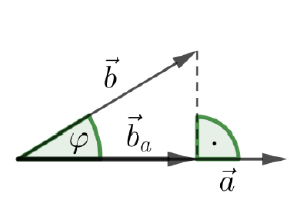
\includegraphics[scale=0.35]{ortho.png}}

        \columnbreak

        $\vec{b}_a = \frac{\vec{a} \cdot  \vec{b}}{\mid \vec{a} \mid ^2} \cdot \vec{a} $

        $\mid \vec{b}_a  \mid  = \frac{\mid \vec{a} \mid \cdot \mid \vec{b} \mid}{\mid \vec{a} \mid }$

        $ \mid \vec{b}_a \mid $ = $\mid \vec{a} \mid \cdot \cos(\varphi)$

    \end{multicols*}

    \subsection{Zwischenwinkel}
    {$\varphi = cos^{-1}(\frac{\vec{a}\cdot\vec{b}}{\mid \vec{a} \mid \cdot \mid \vec{b} \mid}) $}
    \WhiteSpace
    \subsection{Einheitsvektor}
    {$\vec{e}_a $ = $\frac{1}{\mid \vec{a} \mid} \cdot \vec{a}$ ;$\mid \vec{e}_a \mid$ = 1}

    \subsection{Vektorprodukt / Kreuzprodukt}

    \begin{multicols*}{2}

        {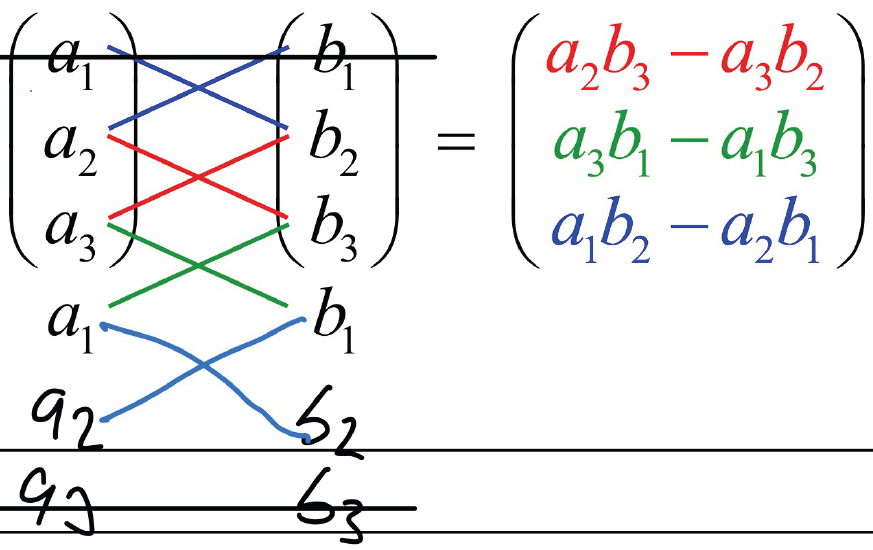
\includegraphics[scale=0.15]{vekProd.png}}

        \columnbreak

        { $ \mid \vec{a} \times \vec{b} \mid = \mid\vec{a}\mid \cdot \mid\vec{b}\mid \cdot \cos(\alpha) $}

        {$\vec{a} \times \vec{b}$ ist orthogonal zu $\vec{a}$ und zu $\vec{b}$}
    
    \end{multicols*}

    \textbf{Fläche / Parallelogramm }
    \begin{multicols*}{2}

        {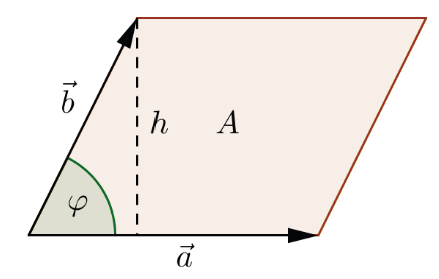
\includegraphics[scale=0.25]{vekProdParallelo.png}}

        \columnbreak

        { $\mid \vec{a} \times \vec{b} \mid $ = A }

        {Dreieck = $\frac{1}{2}$ A}

    \end{multicols*}

    \textbf{Kreuzprodukt in R²}

    { 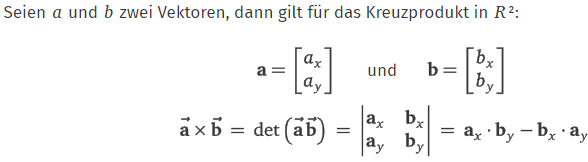
\includegraphics[scale=0.4]{vekProd_r2.png}}


    \WhiteSpace


    \section{Geraden}

    \subsection{Parameterdarstellung}
    {\large $ g: \vec{r}(P) + \lambda \cdot \vec{a}  $}

    {P: Aufpunkt}

    {$ \vec{a}$ = $\overrightarrow{PQ} $;  = Richtungsvektor}


    \subsection{Koordinatendarstellung}
    {$g: ax + by + c= 0 $}
    \subsection{Koordinatendarstellung zu Parameterdarstellung }
    {Zwei Punkte auf $ g $  bestimmen: 2 beliebige x Koordinaten wählen und in $ g $ einsetzen. Danach jeweils $ y $ auslesen. Dies ergibt zwei Punkte $P,Q$. In Parameterdarstellung bringen.}

    \subsection{Parameterdarstellung zu Koordinatendarstellung}
    {Gerade $ g:  \begin{pmatrix}
                7 \\
                1
            \end{pmatrix} + \lambda \cdot \begin{pmatrix}
                -2 \\
                -4
            \end{pmatrix} $ }
    {Gleichungssystem aufstellen und Lösen:}
    \begin{gather*}
        x = 7 - 2 \lambda \\
        y = 1 - 4 \lambda
    \end{gather*}
    {In Koordinatendarstellung bringen:}
    $ -2x + y + 13 = 0$
    \columnbreak
    \subsection{Abstand Punkt zu Geraden}
    { Gerade g: $ \begin{pmatrix}
                1  \\
                13 \\
                -5
            \end{pmatrix} + \lambda \cdot
            \begin{pmatrix}
                3 \\
                5 \\
                -4
            \end{pmatrix} $}

    {Punkt A: $(3,-1,4)$}

    {$\overrightarrow{PA}$ = $\begin{pmatrix}
                3  \\
                -1 \\
                4
            \end{pmatrix} -  \begin{pmatrix}
                1  \\
                13 \\
                -5
            \end{pmatrix} =
            \begin{pmatrix}
                2   \\
                -14 \\
                9
            \end{pmatrix} $}

    {$l = \frac {\mid \overrightarrow{PA} \times\vec{a}\mid}{\mid\vec{a}\mid} $}

    {\small $\vec{a} \Rightarrow $  aus der Parameterdarstellung}
    \section{Ebene}

    \subsection{Normalenvektor der Ebene (orthogonal zur Ebene)}
    {Auf der Ebene $ E $ senkrecht stehnder Vektor $\vec{n}$.}
    $\vec{n} = \vec{a} \times \vec{b}$
    \WhiteSpace
    \subsection{Parameterdarstellung}
    {\large $ E: \vec{r}(P) + \lambda \cdot \vec{a} + \mu \cdot \vec{b} $}
    {P: Aufpunkt}

    {$ \vec{a}$ = $\overrightarrow{PQ} $; $ \vec{b}$ = $\overrightarrow{PR} $ = Richtungsvektoren}
    \WhiteSpace
    \subsection{Koordinatendarstellung}
    {$E: ax + by + cz + d = 0 $}

    \subsection{Parameterdarstellung zu Koordinatendarstellung}
    { $ E: \begin{pmatrix}
                2 \\
                4 \\
                1
            \end{pmatrix} + \lambda \cdot
            \begin{pmatrix}
                1 \\
                3 \\
                1
            \end{pmatrix} + \mu \cdot
            \begin{pmatrix}
                2 \\
                4 \\
                -4
            \end{pmatrix}$

        $\vec{n}=
            \begin{pmatrix}
                1 \\
                3 \\
                1
            \end{pmatrix} \times \begin{pmatrix}
                2 \\
                4 \\
                -4
            \end{pmatrix} = \begin{pmatrix}
                -14 \\
                6   \\
                -4
            \end{pmatrix} $}

    \circled{2} Koordinatendarstellung $ E: -14x + 6y - 4z + d = 0$

    \circled{3} Aufpunkt einsetzen: $\begin{pmatrix}
            2 \\
            4 \\
            1
        \end{pmatrix} 	\Rightarrow  E: -14 \cdot 2  + 6 \cdot 4 - 4\cdot 1 + d = 0 $

    \circled{4} $d$ ausrechnen: $ E: -14 \cdot 2  + 6 \cdot 4 - 4\cdot 1 + d = 0 \Rightarrow d = 8$

    \circled{5} $E: -14x + 6y - 4z + 8 = 0$

    $\Rightarrow \frac{-14x + 6y - 4z + 8 = 0}{2} \Rightarrow E: -7x + 3y - 2z + 4 = 0$
    \WhiteSpace
    \subsection{Koordinatendarstellung zu Parameterdarstellung }
    {Wir bestimmen drei beliebige Punkte auf $ E$, indem wir die $x$- und $y$-Koordinaten frei wählen
        und die zugehörigen $z$-Koordinaten aus der Koordinatendarstellung von $E$ berechnen. Aus
        diesen drei Punkten können wir dann eine Parameterdarstellung von $E$ gewinnen.}
    {$E: 2x + 7y -4z + 1 = 0$}

    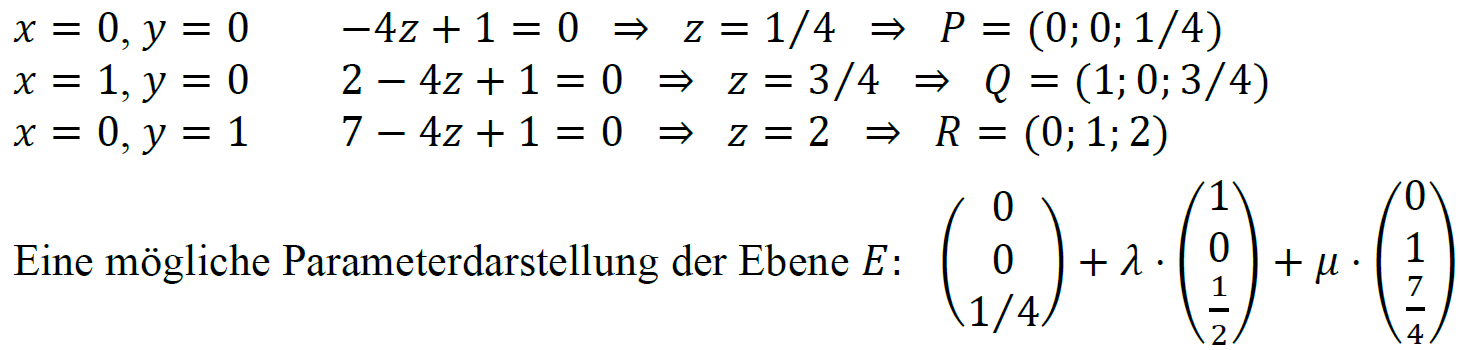
\includegraphics[scale=0.2]{koord_to_param.png}

    \subsection{Abstand Punkt zu Ebene}
    {Abstand \Large $  l = \frac{\mid ax_A + bx_A + cz_A + d  \mid}{\mid \vec{n} \mid}$ }
    {Ebene $E:  3x-6y-2z+67=0 $}

    {Punkt $A = (3,-4,1)$}


    {\circled{1} $\vec{n}$ bestimmen: $\begin{pmatrix}
                3  \\
                -6 \\
                -2
            \end{pmatrix}$ $\sqrt{3^2+-6^2+-2^2} = 7$}

    {\circled{2} $l = \frac{(3 \cdot 3) -(6 \cdot (-4)) - (2 \cdot 1)}{7} = 14$}
    \WhiteSpace
    \subsection{Spezielle Lagen von Ebenen}
    {TBD}

    \subsection{  normierte Koordinatendarstellung der Ebene}
    {$E: 2x + 7y - 4z + 1 = 0$}
    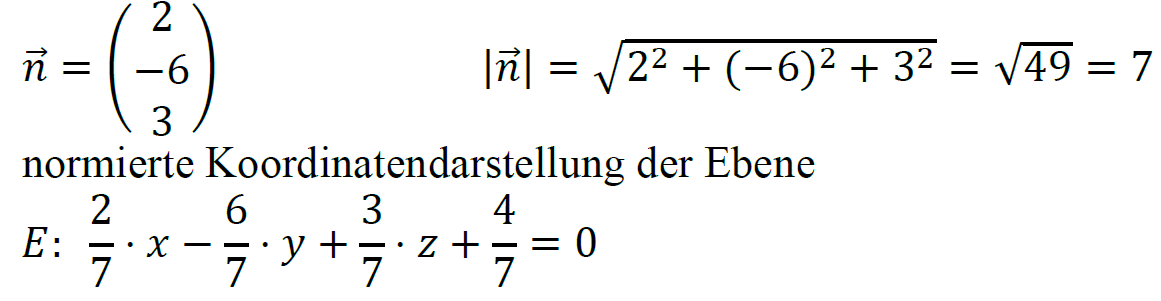
\includegraphics[scale=0.2]{normiert.png}


    \section{Linearen Gleichungssysteme}
    \WhiteSpace
    \subsection{Rang}
    {Matrix muss in Zeilenstufenform sein.}

    {$rg(A) = $ Gesamtanzahl Zeilen - Anzahl Nullzeilen .}

    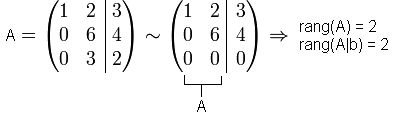
\includegraphics[scale=0.75]{rang.png}

    \subsection{Lösbarkeit von LGS}
    {$ n $ = Anzahl Spalten}
    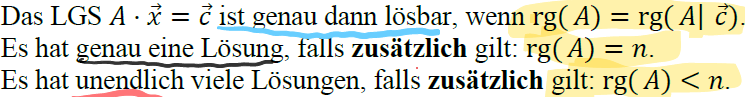
\includegraphics[scale=0.45]{loesbarkeit.png}

    \section{Matrizen}
    \subsection{Begriffe}
    {\textbf{Quadratische Matrix:} gleich viele Zeilen und Spalten}

    \textbf{Hauptdiagonale:} Die Diagonale von links oben nach rechts unten

    \textbf{Untere- und obere Dreiecksmatrix}

    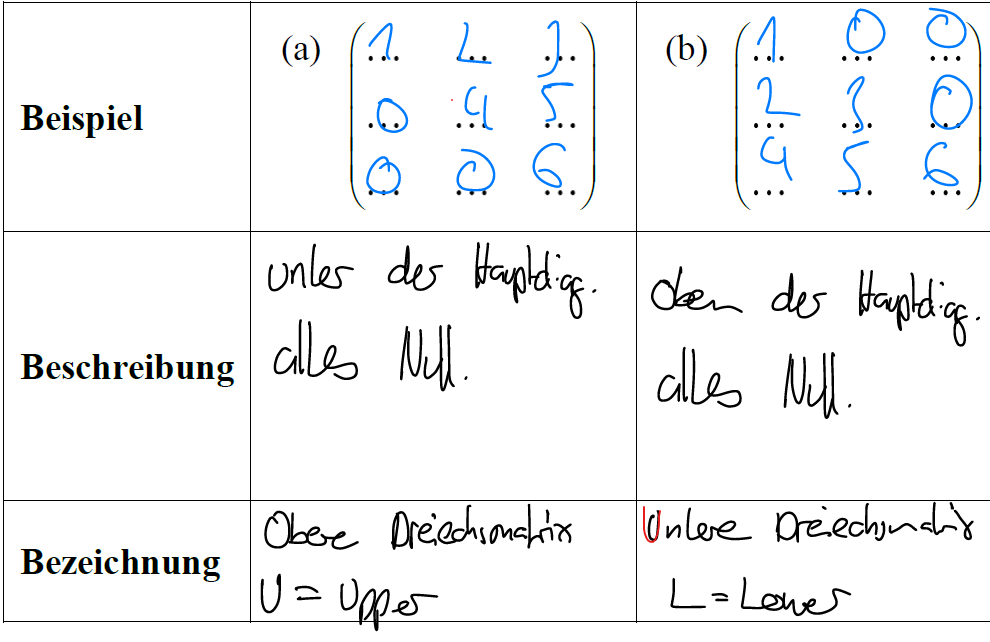
\includegraphics[scale=0.25]{untere_obere.png}

    \textbf{Symmetrische Matrix :} symmetrisch bzgl. Hauptdiagonale

    $ \begin{pmatrix}
            1 & 5 & 6 \\
            5 & 2 & 3 \\
            6 & 3 & 1
        \end{pmatrix} $

    \WhiteSpace
    \subsection{Multiplikation / Rechenregeln}
    {\begin{multicols}{2}
            { 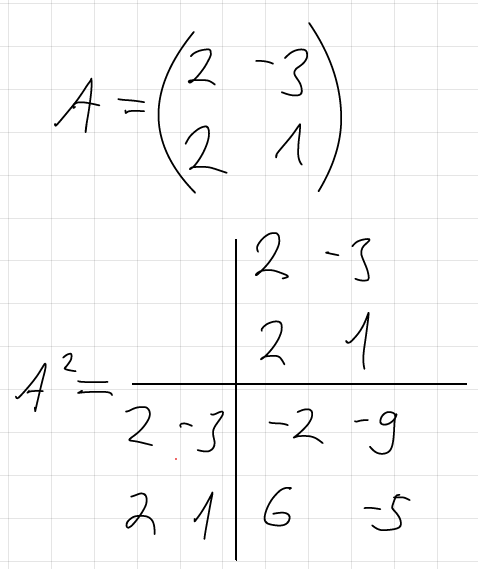
\includegraphics[scale=0.25]{matrix_multi.png} }
            \columnbreak
            { 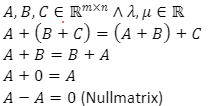
\includegraphics[scale=0.8]{rechenregeln.png} }
        \end{multicols}}

    \subsection{Transponieren}

    A = $\begin{pmatrix} {\color{red}2} & {\color{red}3} & {\color{red}0} \\ 1 & 4 & 5 \end{pmatrix} \quad
        \rightarrow
        \quad A^{T} = \begin{pmatrix} {\color{red}2} & 1 \\ {\color{red}3} & 4 \\ {\color{red}0} & 5 \end{pmatrix}
    $

    {Rechenregeln:}

    $ \left(A^{T}\right)^{T} = A $

    $ \left(A + B\right)^{T} = A^{T} + B^{T} $

    $ \left(A \cdot B\right)^{T} = B^{T} \cdot A^{T} $

    {Gilt $ A = A^{T} $, so heißt die Matrix A symmetrisch.}


    {Gilt $ A = -A^{T} $, so heißt die Matrix A antisymmetrisch.}

    \subsection{Inverse}
    {Matrix muss quadratisch sein$: n \times n \rightarrow 2\times2, 3\times3$}

    \textbf{2x2}

    {\large$\begin{pmatrix}
            a & b \\
            c & d
        \end{pmatrix}^{-1} = \frac{1}{ad-bc}\cdot\begin{pmatrix}
            d  & -b \\
            -c & a
        \end{pmatrix}$}

    {Die $2\times2$-Matrix hat genau dann ein Invese wenn $ad-bc \neq 0$}

    \textbf{3x3 und grösser}

    {$\rightarrow$ Gauss - Jordan}

    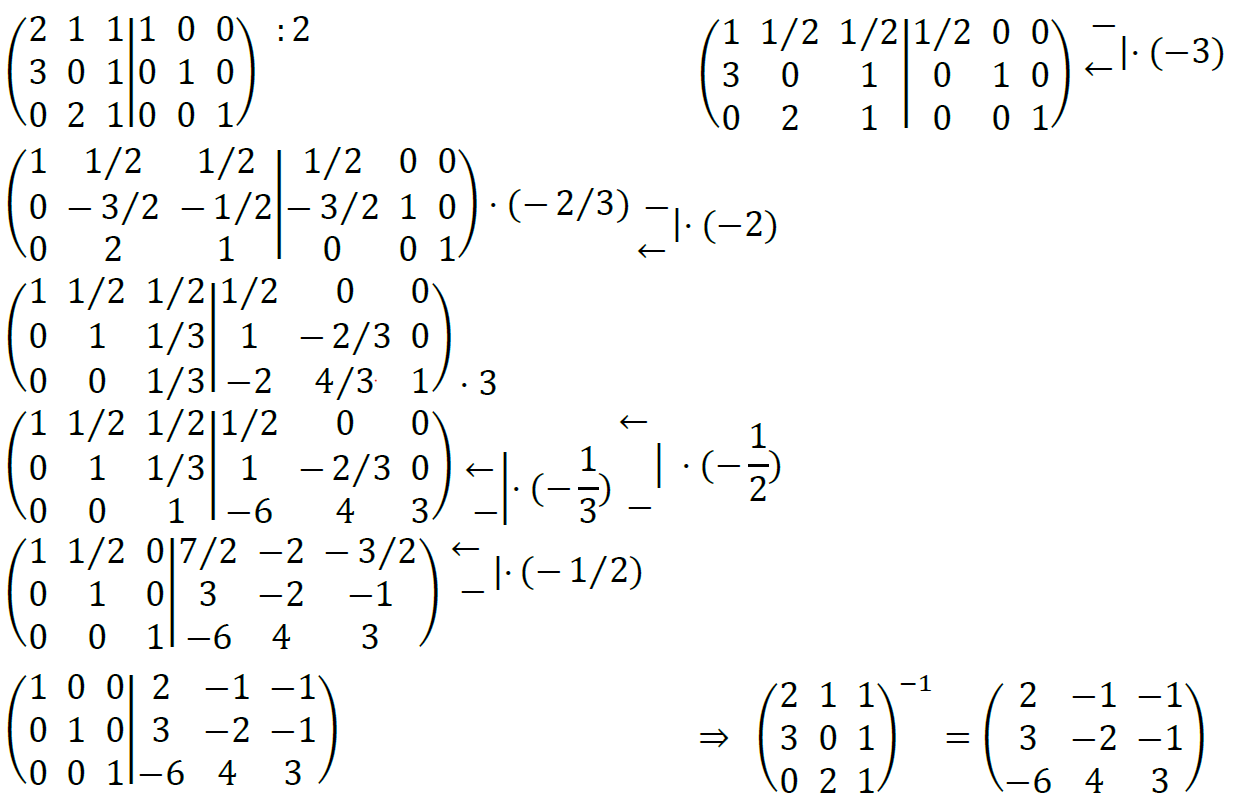
\includegraphics[scale=0.25]{3x3_inverse.png}
    \WhiteSpace

    \subsection{Determinante}
    {\textbf{2x2}}

    $\begin{vmatrix}
            a & b \\
            c & d
        \end{vmatrix} = a\cdot d - b\cdot c $
    \WhiteSpace
    \textbf{3x3 Regel von Sarrus}

    $\begin{vmatrix} a & b & c \\ d & e & f \\ g & h &i \end{vmatrix} = a \cdot e \cdot i + b \cdot f \cdot g + c \cdot d \cdot h - g \cdot e \cdot c - h \cdot f \cdot a - i \cdot d \cdot b.$
    \WhiteSpace
    \textbf{Laplacescher Entwicklungssatz ($ >$3x3)}

    {\begin{multicols}{2}
            Vorzeichen:

            \columnbreak
            { 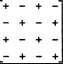
\includegraphics[scale=0.75]{checkerboard.png} }

        \end{multicols}}

    {\small{Entwickeln nach derjenigen Zeile oder Spalte, in
            der die meisten Nullen stehen (hier gelb)}}
    {\begin{multicols}{2}
            {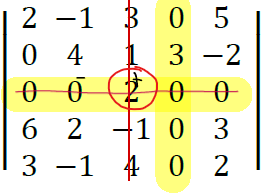
\includegraphics[scale=0.40]{laplace.png}}
            \columnbreak

            {  $ \rightarrow  2 \cdot det \begin{vmatrix} 2 & 1 & 0 & 5 \\ 0 & 4 & 3 & -2 \\ 6 & 2 &0 & 3 \\ 3 & -1 &0 & 2 \end{vmatrix} $}
        \end{multicols}}
    {\small{Wichtig: häufig sind die entwickelten identisch! $\rightarrow$ Aufwand sparen!}}
    {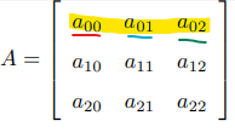
\includegraphics[scale=0.6]{laplace_full_1.png}Entwicklen nach 1er}

    {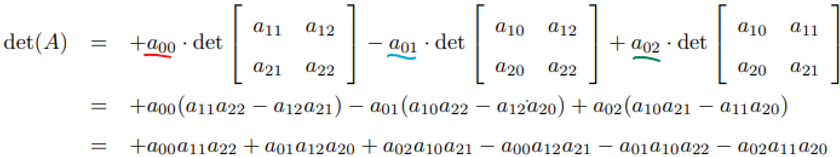
\includegraphics[scale=0.4]{laplace_full_2.png}}


    \textbf{$det$ Dreiecksmatrix}
    $ = $ Produkt der Hauptdiagonale
    \WhiteSpace

    \textbf{Rechenregeln}

    {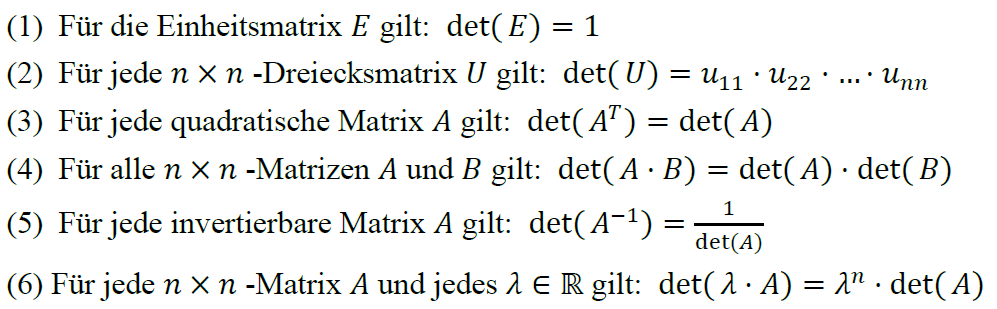
\includegraphics[scale=0.3]{det.png}}

    $2\times 2 \rightarrow det(5 \cdot A) = 5^2 \cdot det(A)$

    $3\times 3 \rightarrow det(5 \cdot A) = 5^3 \cdot det(A)$

    \WhiteSpace
    \subsection{Geometrische Interpretation der Determinante }
    {\textbf{2x2}}

    {Fläche von $\vec{a} $ und $ \vec{b} = $ Betrag von $ det \begin{vmatrix} a1 & b1  \\ a2 & b2 \end{vmatrix} $}
    {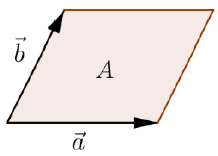
\includegraphics[scale=0.2]{2x2_det_geom.png}}




    \textbf{3x3}

    {Volumen von $\vec{a} $, $ \vec{b}$ und $\vec{c} = $ Betrag von $   det \begin{vmatrix} a1 & b1 & c1 \\ a2 & b2 & c2 \\ a3 & b3 & c3  \end{vmatrix}  $}
    {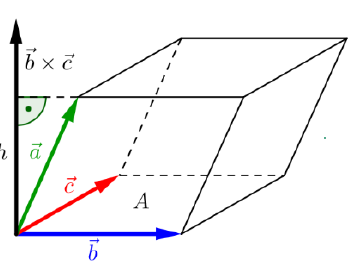
\includegraphics[scale=0.2]{3x3_det_geom.png}}
    \mbox{}


    \section{Linearen Gleichungssysteme}
    \subsection{Rang}
    {Matrix muss in Zeilenstufenform sein.}

    {$rg(A) = $ Gesamtanzahl Zeilen - Anzahl Nullzeilen .}

    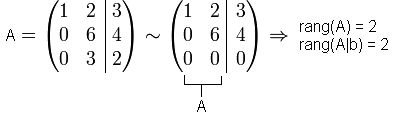
\includegraphics[scale=0.75]{rang.png}

    \subsection{Lösbarkeit von LGS}

    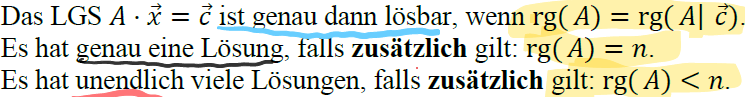
\includegraphics[scale=0.45]{loesbarkeit.png}

    \subsection{Freie Variable}

    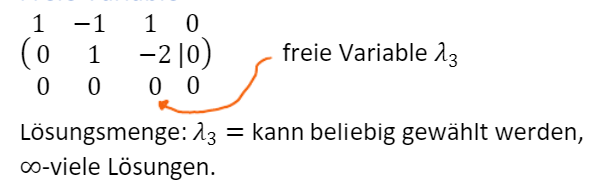
\includegraphics[scale=0.75]{free_vars.png}


    \section{Vektorräume}

    \subsection{Unterräume}
    {Eine Teilmenge U eines Vektorraums V heisst Unterraum von V wenn U selber auch ein Vektorraum ist.}

    {Unterraumkriterien}

    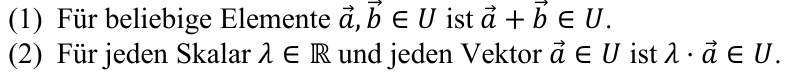
\includegraphics[scale=0.75]{unterkrit.png}

    \subsection{Nullvektorraum}


\end{multicols*}

\end{document}
